\documentclass{article}
\usepackage{graphicx}
\usepackage{lipsum}
\usepackage{enumitem}
\usepackage{fancyhdr}
\usepackage{setspace}


\pagestyle{fancy}
\fancyhf{}
\rhead{Ayrton y Lorenzo Bregant} % Texto en el encabezado a la derecha
\lhead{CS} % Texto en el encabezado a la izquierda

\title{
	
\includegraphics[width=0.6\linewidth]{imagenes/logo.png}\\[1.5em]
	Práctica Profesional I - Trabajo Final
}
\author{\\ \\ \\ Alumnos: Ayrton M. Bregant, Lorenzo Bregant \\ \\ Carrera: Técnico Superior en Desarrollo de Software \\ \\ Proyecto: Trabajo Final PPI \\ \\ Año cursado: 2do}
\date{}

\setstretch{1.5}
\begin{document}

\maketitle
\clearpage
\section{Introducción}
\parindent=2 em


	   En respuesta a la creciente necesidad de optimización de recursos en la industria metalúrgica, ha surgido 'CS' como una solución integral diseñada de manera específica para satisfacer las demandas de fábricas metalúrgicas. Este trabajo final se centra en una documentación exhaustiva de 'CS', un software que permitirá una gestión integral del circuito productivo en su totalidad, desde la compra de insumos para la fabricación de las máquinas, incluyendo la gestión de proveedores hasta la gestión de clientes y los pedidos realizados por estos. A su vez, permitirá gestionar el stock tanto de los insumos (piezas y materiales) necesarios para la fabricación de las máquinas, como así también de las máquinas fabricadas.
	
	   Nuestra elección de estudio de caso recae en "Avila Maquinarias", una empresa familiar con varios empleados que, hasta el momento, ha carecido de un sistema de control de inventario, dependiendo en su lugar de hojas de cálculo y documentos impresos para gestionar su información.
	
	   En las siguientes páginas, explicaremos en detalle las características esenciales de 'CS', su funcionamiento y su potencial para transformar la gestión de inventario en la industria metalúrgica. Además, se proporcionarán directrices claras para su implementación y uso efectivo. A medida que avanzamos, descubriremos cómo 'CS' se convierte en un aliado estratégico, mejorando la eficiencia de la producción y contribuyendo a la rentabilidad de las fábricas metalúrgicas en un entorno altamente competitivo.

\section{Abstract}
	
	   In response to the growing need for resource optimization in the metallurgical industry, 'CS' has emerged as a comprehensive solution specifically designed to meet the demands of metallurgical factories. This final work focuses on a comprehensive documentation of 'CS,' a software that will enable comprehensive management of the entire production process, from the purchase of raw materials for machine manufacturing, including supplier management to customer management and orders placed by them. Furthermore, it will allow for the management of both the stock of the raw materials (parts and materials) required for machine manufacturing, as well as the machines manufactured.
	
	   Our case study choice falls on "Avila Maquinarias," a family-owned company with several employees that, until now, has lacked an inventory control system, relying instead on spreadsheets and printed documents to manage their information.

	   In the following pages, we will explain in detail the essential features of 'CS', how it operates, and its potential to transform inventory management in the metallurgical industry. Furthermore, clear guidelines for its implementation and effective use will be provided. As we progress, we will discover how 'CS' becomes a strategic ally, improving production efficiency and contributing to the profitability of metallurgical factories in a highly competitive environment.

\section{Descripción del sistema}

	   El sistema planteado para Ávila Maquinarias permite al usuario una gestión integral y eficiente de todo el circuito productivo en la industria metalúrgica.
	
	   Conocido como 'CS', este software se enfoca en optimizar recursos desde la compra de insumos hasta la entrega de productos a clientes. Su funcionalidad abarca la gestión de proveedores, el control en tiempo real del inventario de insumos y productos fabricados, así como la administración de clientes y pedidos. 

	   El sistema permite llevar un control de los insumos necesarios para la fabricación de una máquina. Cuando se selecciona una máquina, automáticamente se da de baja la cantidad de materia prima que conlleva dicha máquina. Ej: si una máquina utiliza 2 rodamientos, se descontarán esos dos rodamientos de la lista de materiales.

	   Además, el sistema emite una alerta cuando la cantidad de materiales llega a cierto punto de escasez para así poder hacer el pedido a los proveedores.
	
	   El software también mantiene un registro detallado de los pedidos de máquinas realizados por los clientes, teniendo en cuenta la posibilidad de cancelaciones, suspensiones o entregas.

\section{Requerimientos}
\subsection{Funcionales}

\begin{itemize}
	\item Gestión de insumos
	\begin{enumerate}
		\item Ingresar insumos.
		\item Modificar registros de insumos.
		\item Eliminar registros de insumos.
		\item Categorizar materiales (Chapas y Redondos, Gases, Insumos Varios, Aceites).
		\item Mantener una lista actualizada de insumos utilizados en la producción.
	\end{enumerate}
\end{itemize}

\begin{itemize}
	\item Gestión de proveedores
	\begin{enumerate}[start=6]
		\item Registrar la entrada de nuevos materiales.
		\item Registrar la salida de materiales.
		\item Asignar responsables para estas transacciones.
	\end{enumerate}
\end{itemize}

\begin{itemize}
	\item Relación entre Materiales y Máquinas
	\begin{enumerate}[start=9]
		\item Listar qué materiales se utilizan en la producción de máquinas específicas.
		\item Registrar la cantidad de cada material utilizado en cada máquina.
		\item Generar alertas por bajo stock de materiales necesarios para la producción de máquinas.
	\end{enumerate}
\end{itemize}

\begin{itemize}
	\item Gestión de productos
	\begin{enumerate}[start=12]
		\item Ingresar máquinas.
		\item Modificar registros de máquinas.
		\item Eliminar registros de máquinas.
		\item Consultar el inventario de máquinas.
	\end{enumerate}
\end{itemize}

\begin{itemize}
	\item Gestión de clientes
	\begin{enumerate}[start=16]
		\item Ingresar clientes.
		\item Modificar registro de clientes.
	\end{enumerate}
\end{itemize}

\begin{itemize}
	\item Gestión de pedidos (Distintos estados: Pendiente, en preparación, terminado y entregado)
	\begin{enumerate}[start=18]
		\item Registrar pedido.
		\item Modificar pedido.
		\item Cancelar Pedidos.
	\end{enumerate}
\end{itemize}

\begin{itemize}
	\item Gestión de compras (comprar insumos).
	\begin{enumerate}[start=21]
		\item Registrar Lista de Compra
	\end{enumerate}
\end{itemize}

\subsection{No funcionales}
\begin{enumerate}
	\item Usabilidad
	\begin{itemize}
		\item La interfaz de usuario debe ser intuitiva y fácil de usar, de modo que los usuarios puedan aprender a utilizar el sistema con rapidez.
	\end{itemize}
\end{enumerate}

\begin{enumerate}[start=2]
	\item Rendimiento
	\begin{itemize}
		\item El sistema debe ser capaz de manejar grandes volúmenes de datos sin demoras significativas.
		\item El tiempo de respuesta del sistema no debe exceder los X segundos para ninguna operación.
	\end{itemize}
\end{enumerate}

\clearpage
\begin{enumerate}[start=3]
	\item Seguridad
	\begin{itemize}
		\item El acceso al sistema debe estar protegido por contraseñas seguras y autenticación de usuarios.
	\end{itemize}
\end{enumerate}

\begin{enumerate}[start=4]
	\item Disponibilidad
	\begin{itemize}
		\item El sistema debe estar disponible para su uso las 24 horas del día, los 7 días de la semana, con un tiempo de inactividad planificado mínimo para mantenimiento.
	\end{itemize}
\end{enumerate}

\begin{enumerate}[start=5]
	\item Escalabilidad
	\begin{itemize}
		\item El sistema debe ser escalable para acomodar un aumento en el número de usuarios y registros de inventario.
	\end{itemize}
\end{enumerate}

\begin{enumerate}[start=6]
	\item Compatibilidad
	\begin{itemize}
		\item El software debe ser compatible con los sistemas operativos utilizados en la fábrica (en este caso, Windows 10).
	\end{itemize}
\end{enumerate}

\begin{enumerate}[start=7]
	\item Backup y Recuperación
	\begin{itemize}
		\item Debe implementarse un sistema de copias de seguridad regular para garantizar la recuperación de datos en caso de pérdida o fallo del sistema.
	\end{itemize}
\end{enumerate}

\section{Diagramas de casos de uso}
	\begin{center}
		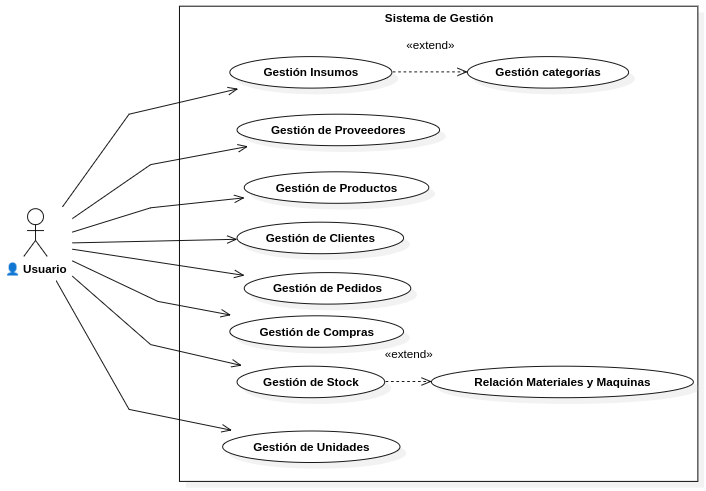
\includegraphics[width=1\linewidth]{imagenes/cu_sistema_de_gestion.png}
		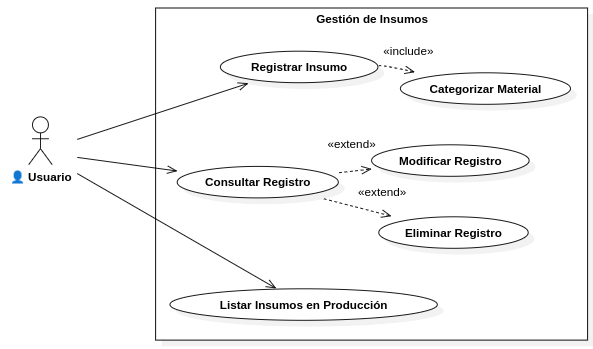
\includegraphics[width=1\linewidth]{imagenes/cu_gestion_de_insumos.png}
		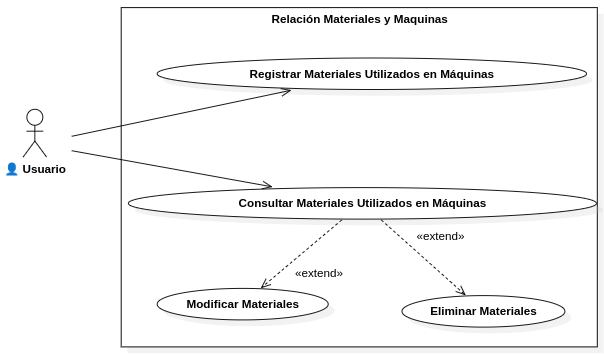
\includegraphics[width=1\linewidth]{imagenes/cu_relacion_materiales_maquinas.png}
	\end{center}

\section{Especificación de casos de uso}
<<<<<<< HEAD
	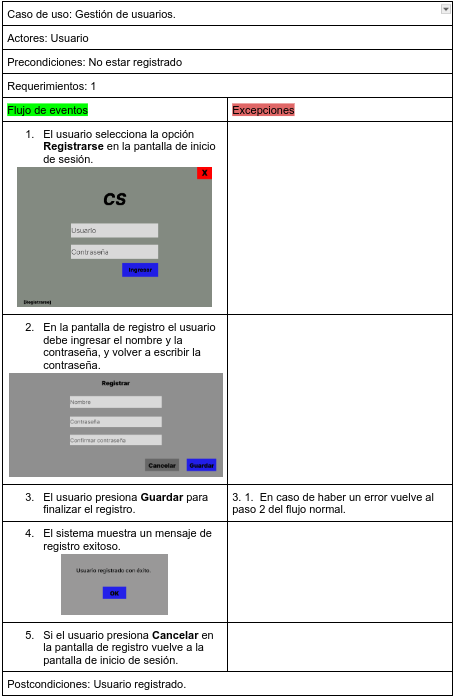
\includegraphics[width=0.95\linewidth]{imagenes/especificacion_usuario.png}
=======
	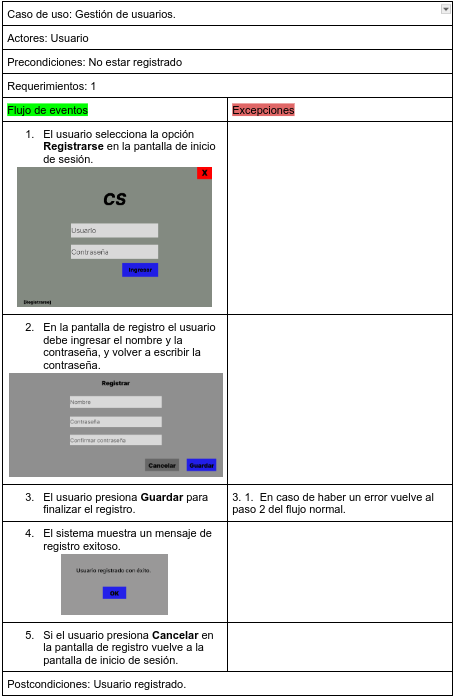
\includegraphics[width=1\linewidth]{imagenes/especificacion_usuario.png}
	
	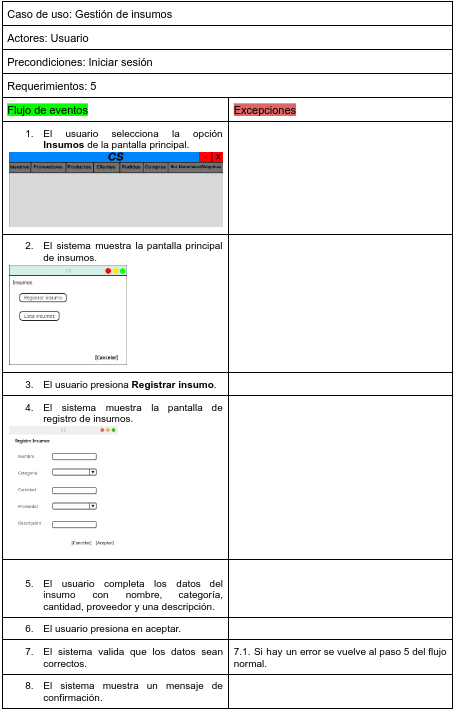
\includegraphics[width=1\linewidth]{imagenes/especificacion_insumos.png}
	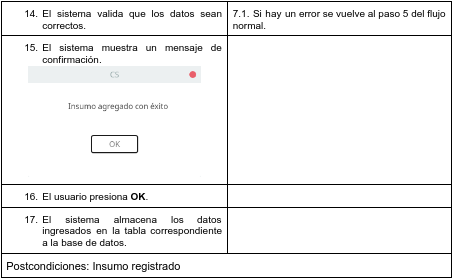
\includegraphics[width=1\linewidth]{imagenes/especificacion_insumos2.png}
>>>>>>> 6dbd0423e84765ed2016ef42166cfe5baef8afa1

    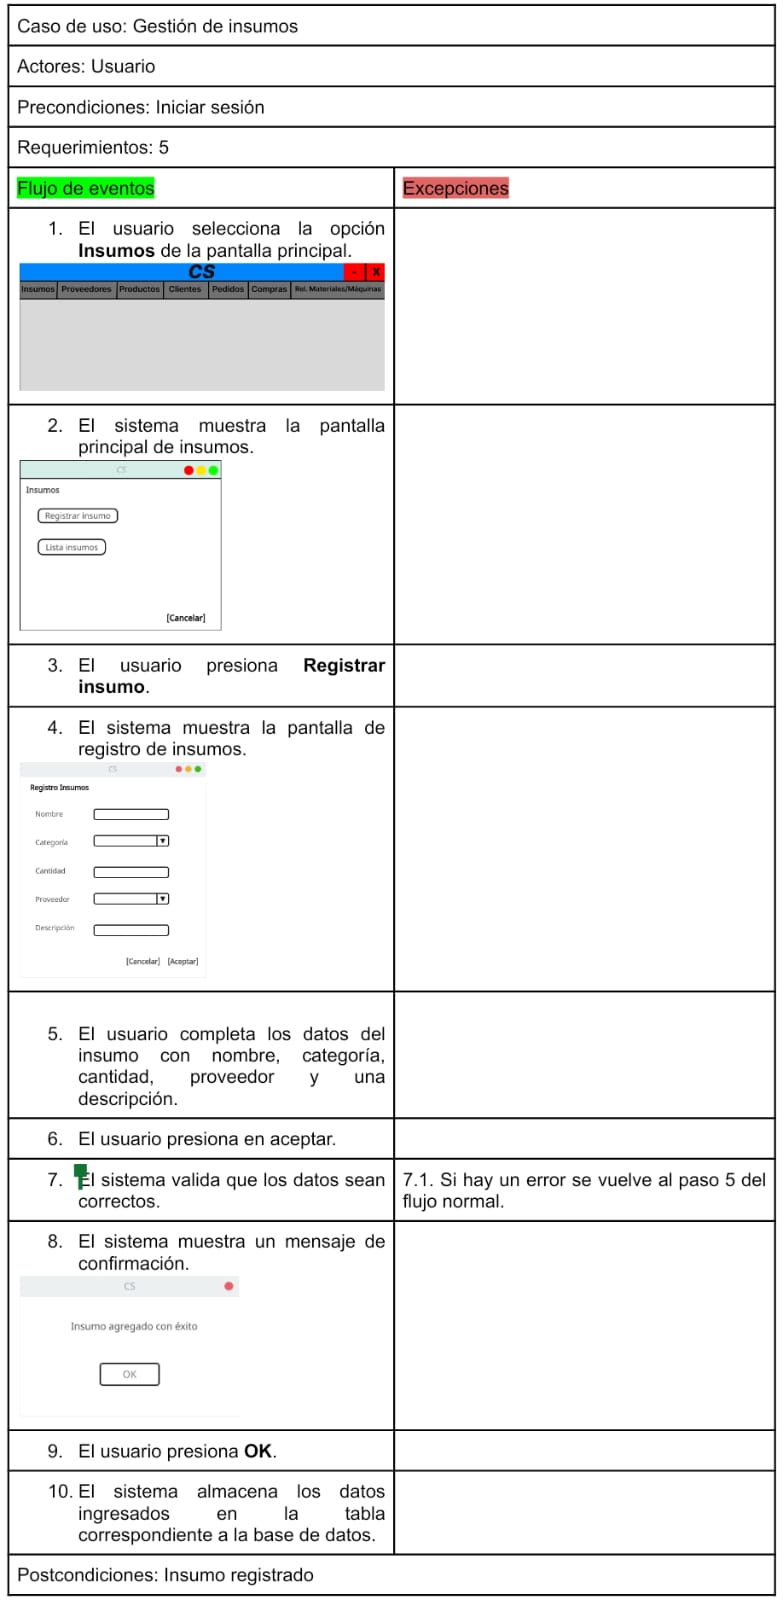
\includegraphics[width=0.9\linewidth]{imagenes/imagen_de_especificaion_muy_dificil_de_replicar_en_latex.jpg}

    \begin{figure}
        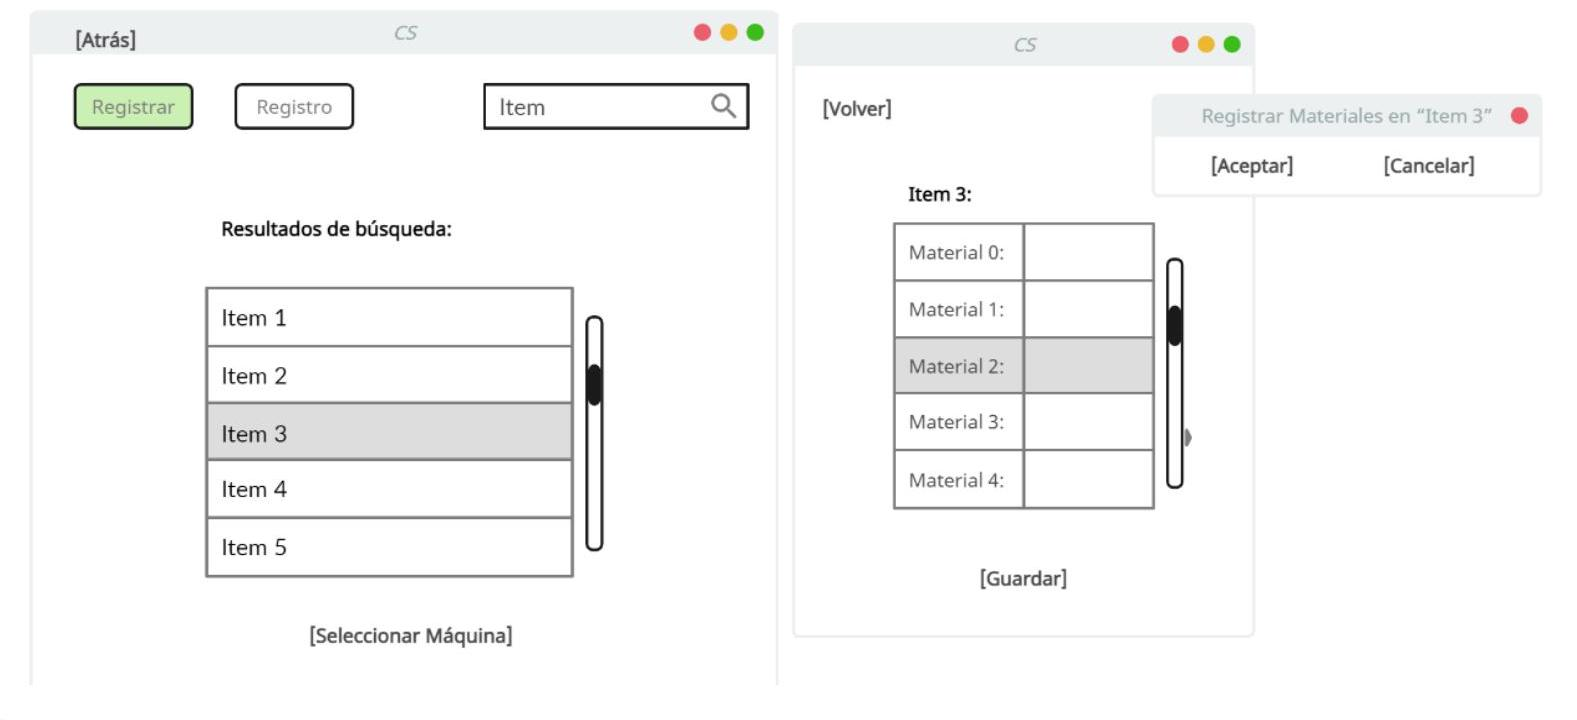
\includegraphics[width=1\linewidth]{imagenes/pan_registrar_materialespormaquina.png}
        \caption{Pantallas R13}
    \end{figure} 
    
    \begin{figure}
        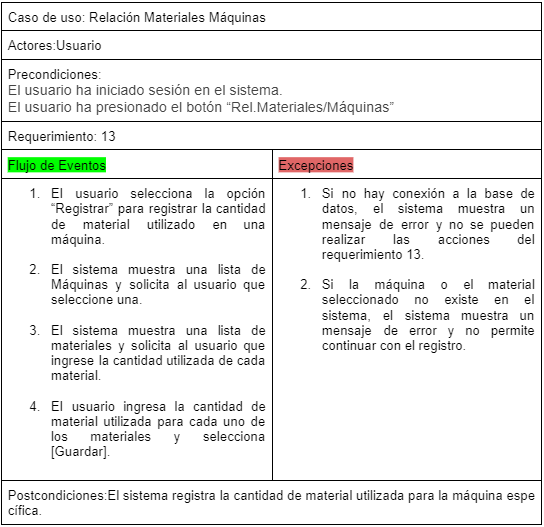
\includegraphics[width=0.9\linewidth]{imagenes/img_diagram_usecase.png}  
    \end{figure}
    
    \begin{figure}
        \begin{center}
            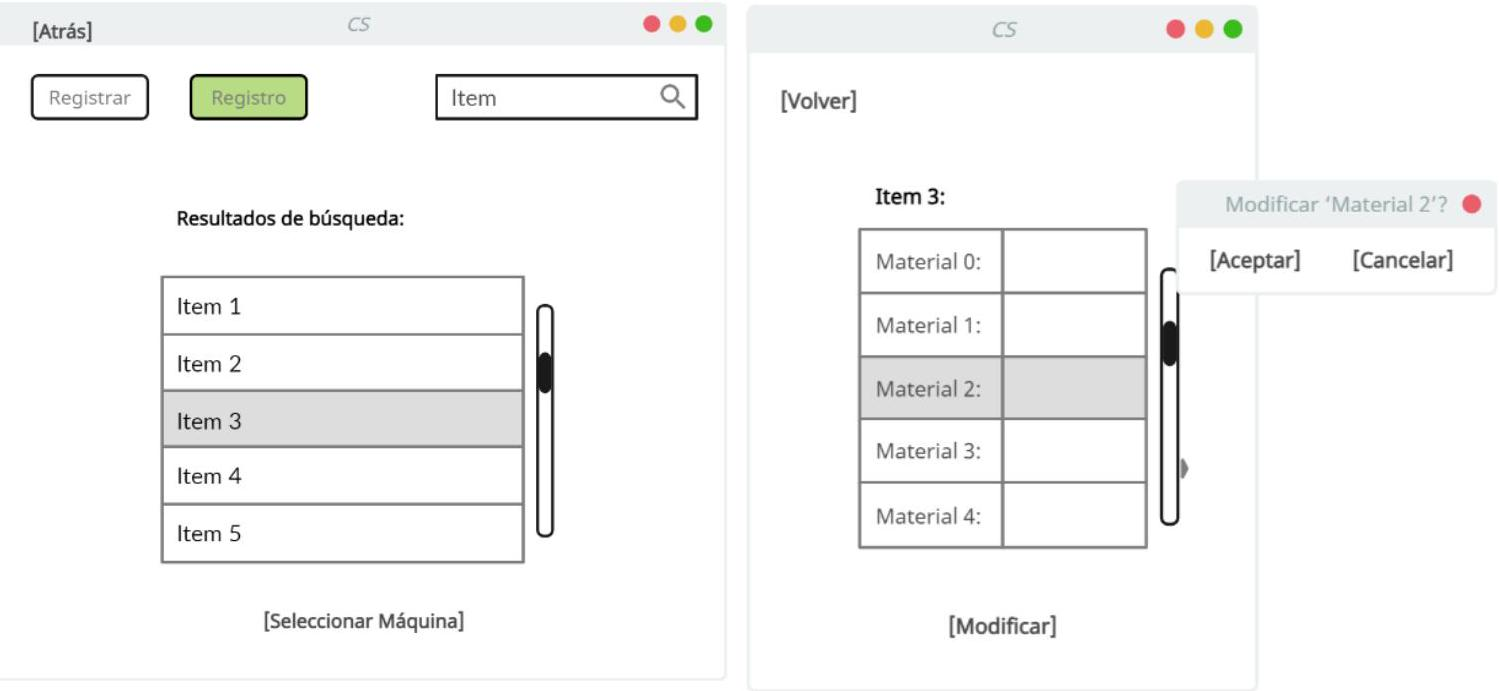
\includegraphics[width=0.9\linewidth]{imagenes/pan_registro_lista-modificar.jpg}
            \caption{Pantallas R14}
        \end{center}
    \end{figure}
    
    \begin{figure}
        \begin{center}
            \includegraphics[width=0.9\linewidth]{imagenes/Buscar-Máquina-Registrar.png}  
        \end{center}
    \end{figure}
    
    \begin{figure}
        \begin{center}
            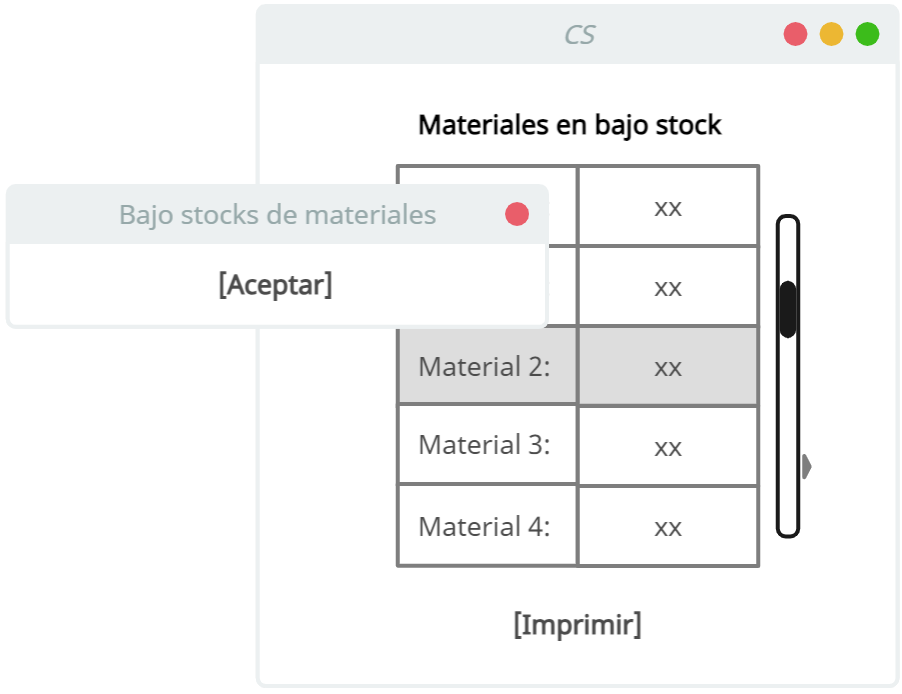
\includegraphics[width=0.8\linewidth]{imagenes/pan_alerta.png}
            \caption{Pantallas R15}  
        \end{center}
    \end{figure}
    
    \begin{figure}
        \begin{center}
            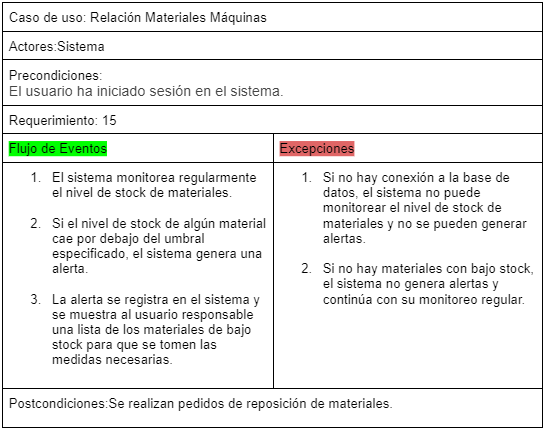
\includegraphics[width=1\linewidth]{imagenes/diagram_usecase_alert_bajostocks.png}  
        \end{center}  
    \end{figure}
    
\clearpage

\section{Entrevista}
    \begin{enumerate}
        \item Gestión Actual de Stocks:
            \begin{enumerate}[label=\Alph*.]
                \item[a.] ¿Cómo gestionan actualmente el inventario de materiales y máquinas en su fábrica? \\
                    Con hojas de cálculo individuales, cada máquina tiene su registro.
                \item[b.] ¿Utilizan algún software o sistema para llevar un registro de los stocks o es principalmente manual? \\
                    Excel
                \item[c.] ¿Cuáles son las dificultades que enfrentan con la forma de gestionar el inventario hoy en día? \\
                    Poco práctico, atento a que falten piezas en la máquina, pérdida de tiempo. 
                \item[d.] ¿Qué sistema operativo utiliza? \\
                    Windows 10
            \end{enumerate}
    \end{enumerate}
    
    \begin{enumerate}[start=2]
        \item Tipos de Materiales:
            \begin{enumerate}[label=\Alph*.]
            \item[a.]  ¿Podría proporcionar una lista de insumos utilizados en la producción? \\
                Acero aisi 304 (chapas, caños, redondos, etc), plástico de ingeniería (grillon, etc), SAE 1010, 1045, motores y reductores, poleas, engranajes, correas, cadenas, rodamientos, retenes, cables, discos, elementos eléctricos (llaves, contactores, etc), gases industriales (argón y oxígeno), consumibles para plasma (electrodo, toberas y escudo), consumibles para torno (porta e insertos).
            \item[b.]  ¿Cómo se categorizan los insumos? \\       
                CHAPAS Y REDONDOS (KG) GASES (mts3) INSUMOS VARIOS (UNIDAD) ACEITES (Lts)
            \end{enumerate}
    \end{enumerate}

    \begin{enumerate}[start=3]
        \item Entrada y Salida de Materiales:
            \begin{enumerate}[label=\Alph*.]
                \item[a.]  ¿Cómo se registra la entrada de nuevos materiales en su fábrica? \\
                    De ninguna forma, solo revisando el remito de los proveedores.
                \item[b.] ¿Qué proceso siguen para registrar la salida de materiales? \\
                	Actualmente ninguno.
                \item[c.] ¿Quiénes son los responsables de realizar estas transacciones? \\
                    Varios usuarios, con su propio nombre y contraseña.
            \end{enumerate}
    \end{enumerate}

    \begin{enumerate}[start=4]
        \item Relación entre Materiales y Máquinas:
            \begin{enumerate}[label=\Alph*.]
                \item[a.] ¿Cómo se determina qué materiales se utilizan en la producción de máquinas específicas? \\
                    Previo diseño y posteriormente en los planos.
                \item[b.]  ¿Existe un registro de cuánto de cada material se utiliza en cada máquina? \\
                    Sí, en excel.
                \item[c,] ¿Cómo la cantidad de inventario de materiales afecta al haber poco en existencia? \\
                    Número mínimos (advertencia de poco stock)Cuando hay números mínimos (ej. 100 tornillos) se lanzaría una advertencia de poco stock.
            \end{enumerate}
    \end{enumerate}

    \begin{enumerate}[start=5]
        \item Control de Máquinas:
            \begin{enumerate}[label=\Alph*.]
                \item[a.] ¿Cómo gestionan el inventario de máquinas en su fábrica? \\
                    En excel.
                \item[b.] ¿Se realiza algún seguimiento de la utilización de las máquinas? \\
                    No
                \item[c.] ¿Qué información importante necesita mantenerse sobre el estado de las máquinas? \\
                    Año de fabricación.
            \end{enumerate}
    \end{enumerate}

    
\end{document}